
%(BEGIN_QUESTION)
% Copyright 2011, Tony R. Kuphaldt, released under the Creative Commons Attribution License (v 1.0)
% This means you may do almost anything with this work of mine, so long as you give me proper credit

This pressure control system has a problem.  Both the indicating controller (PIC) and the pressure gauge (PG) show zero inches WC pressure, even though the controller is in manual mode with 100\% output.  A voltmeter connected between terminals 6 and 7 registers 24 VDC:

$$\includegraphics[width=15.5cm]{i01794x01.eps}$$

Identify the likelihood of each specified fault for this circuit.  Consider each fault one at a time (i.e. no coincidental faults), determining whether or not each fault could independently account for {\it all} measurements and symptoms in this circuit.

% No blank lines allowed between lines of an \halign structure!
% I use comments (%) instead, so that TeX doesn't choke.

$$\vbox{\offinterlineskip
\halign{\strut
\vrule \quad\hfil # \ \hfil & 
\vrule \quad\hfil # \ \hfil & 
\vrule \quad\hfil # \ \hfil \vrule \cr
\noalign{\hrule}
%
% First row
{\bf Fault} & {\bf Possible} & {\bf Impossible} \cr
%
\noalign{\hrule}
%
% Another row
250 ohm resistor failed open &  &  \cr
%
\noalign{\hrule}
%
% Another row
PY (I/P transducer) coil failed open &  &  \cr
%
\noalign{\hrule}
%
% Another row
Wire open between terminal 3 and ($-$) terminal on PT &  &  \cr
%
\noalign{\hrule}
%
% Another row
Wire open between terminal 6 and (+) terminal on PIC &  &  \cr
%
\noalign{\hrule}
%
% Another row
Wire open between terminal 3 and (+) terminal on PIC &  &  \cr
%
\noalign{\hrule}
%
% Another row
Wire open between terminal 7 and ($-$) terminal on PY &  &  \cr
%
\noalign{\hrule}
%
% Another row
24 VDC power supply dead &  &  \cr
%
\noalign{\hrule}
} % End of \halign 
}$$ % End of \vbox

\underbar{file i01794}
%(END_QUESTION)





%(BEGIN_ANSWER)

% No blank lines allowed between lines of an \halign structure!
% I use comments (%) instead, so that TeX doesn't choke.

$$\vbox{\offinterlineskip
\halign{\strut
\vrule \quad\hfil # \ \hfil & 
\vrule \quad\hfil # \ \hfil & 
\vrule \quad\hfil # \ \hfil \vrule \cr
\noalign{\hrule}
%
% First row
{\bf Fault} & {\bf Possible} & {\bf Impossible} \cr
%
\noalign{\hrule}
%
% Another row
250 ohm resistor failed open &  & $\surd$ \cr
%
\noalign{\hrule}
%
% Another row
PY (I/P transducer) coil failed open & $\surd$ &  \cr
%
\noalign{\hrule}
%
% Another row
Wire open between terminal 3 and ($-$) terminal on PT &  & $\surd$ \cr
%
\noalign{\hrule}
%
% Another row
Wire open between terminal 6 and (+) terminal on PIC &  & $\surd$ \cr
%
\noalign{\hrule}
%
% Another row
Wire open between terminal 3 and (+) terminal on PIC &  & $\surd$ \cr
%
\noalign{\hrule}
%
% Another row
Wire open between terminal 7 and ($-$) terminal on PY & $\surd$ &  \cr
%
\noalign{\hrule}
%
% Another row
24 VDC power supply dead &  & $\surd$ \cr
%
\noalign{\hrule}
} % End of \halign 
}$$ % End of \vbox

%(END_ANSWER)





%(BEGIN_NOTES)

{\bf This question is intended for exams only and not worksheets!}.

%(END_NOTES)


